%!TEX root = ../report.tex

\section{Experiments}

\begin{itemize}
    \item Describe experiments and compare with results in the paper.
\end{itemize}

\subsection{Simulated examples}

\subsection{Bayesian Neural Networks for Classification}
For the Bayesian neural network (BNN) MNIST classification we actually used the reparameterisation of SGHMC described in the section ``Connection to SGD with Momentum'' of \cite{sghmc}. The SGHMC algorithm is reframed in terms of learning rate and momentum decay, and simulates the following dynamics instead:
$$\begin{cases}
\nabla \theta = v\\
\nabla v = - \eta \nabla \wt{U}(\theta) - \alpha v + \mathcal{N}(0, 2(\alpha - \wh{\beta}) \eta)
\end{cases}
$$
where $\eta = \epsilon^2 M^{-1}, \alpha = \epsilon M^{-1}C, \wh{\beta} = \eta M^{-1}\wh{B}$. In all our experiments in this section we set the mass matrix $M $ to the identity, and the noise model $\wh{\beta} = \wh{B} = 0$. Other than the architecture of the BNN there are now only 3 hyperparameters for SGHMC, the learning rate $\eta$, the momentum decay $\alpha$ and the batch size $|\wt{\D}|$, in all our experiments we fixed $|\wt{\D}| = 500$ which follows from \cite{sghmc}.

To build on top of the work in \cite{sghmc} we implemented learning rate annealing for SGLD and following \cite{sgld} we weighted the samples by the learning rate as follows:
$$\mathbb{E}[f(\theta)] \approx \frac{\sum^T_{t=1} \epsilon_t f(\theta_t)}{\sum^T_{t=1} \epsilon_t}$$
Although since $f$ is a classifier we can ignore the denominator. Our BNN followed the same architecture as in \cite{sghmc}, that is one linear with 100 hidden units followed by ReLU activation followed by another linear layer and a log softmax for multi-class classification. The weights and biases for both linear layers are sampled from univariate standard normal distributions, but the Pyro method \texttt{to\_event()} declares dependence between the parameters. 

Our implementations of SGD and SGD with momentum are meant to be used directly with Pyro, and so Gaussian priors on the weights and biases is equivalent to L2 regularization in the non-Bayesian paradigm. We experimented with regularization strengths of $\lambda \in \{0.1, 1.0, 10.0\}$ and found $\lambda = 1.0$ to be the most effective. Additionally we implemented weight decay for both SGD and SGD with momentum but found that this didn't improve anything in this setting.

For the momentum based algorithms, SGHMC and SGD with momentum, we tried $\eta \in \{1.0, 2.0, 4.0, 8.0 \} \times 10^{-6}$, and $\alpha \in \{0.1, 0.01, 0.001 \}$. For SGHMC the best configuration was $\eta = 2.0\time10^{-6}, \alpha=0.01$, and for SGD with momentum the best configuration was $\eta = 1.0\time10^{-6}, \alpha=0.01$.

For SGLD and SGD, we tried $\eta \in \{1.0, 2.0, 4.0, 6.0\} \times 10^{-5}$, for SGLD we also tried learning rate annealing but it proved not to make much of a difference in this setting so we ignored it in the end. The best configuration for SGLD was $\eta = 4.0\time10^{-5}$, and for SGD the best configuration was $\eta = 1.0\times10^{-5}$.

For MNIST we ran each of the algorithms for 800 epochs with 50 warmup epochs. For the sampling algorithms we do Bayesian averaging over all the sampled parameterisations of the BNN after warmup as is described in Section II of \cite{hands-on-bnn} and report the test error. For the optimization algorithms we take most recent sample / set of parameters as a point estimate and report the test error.  Figure \ref{fig:MNIST} presents our results.

\begin{figure}[h!]
\centering
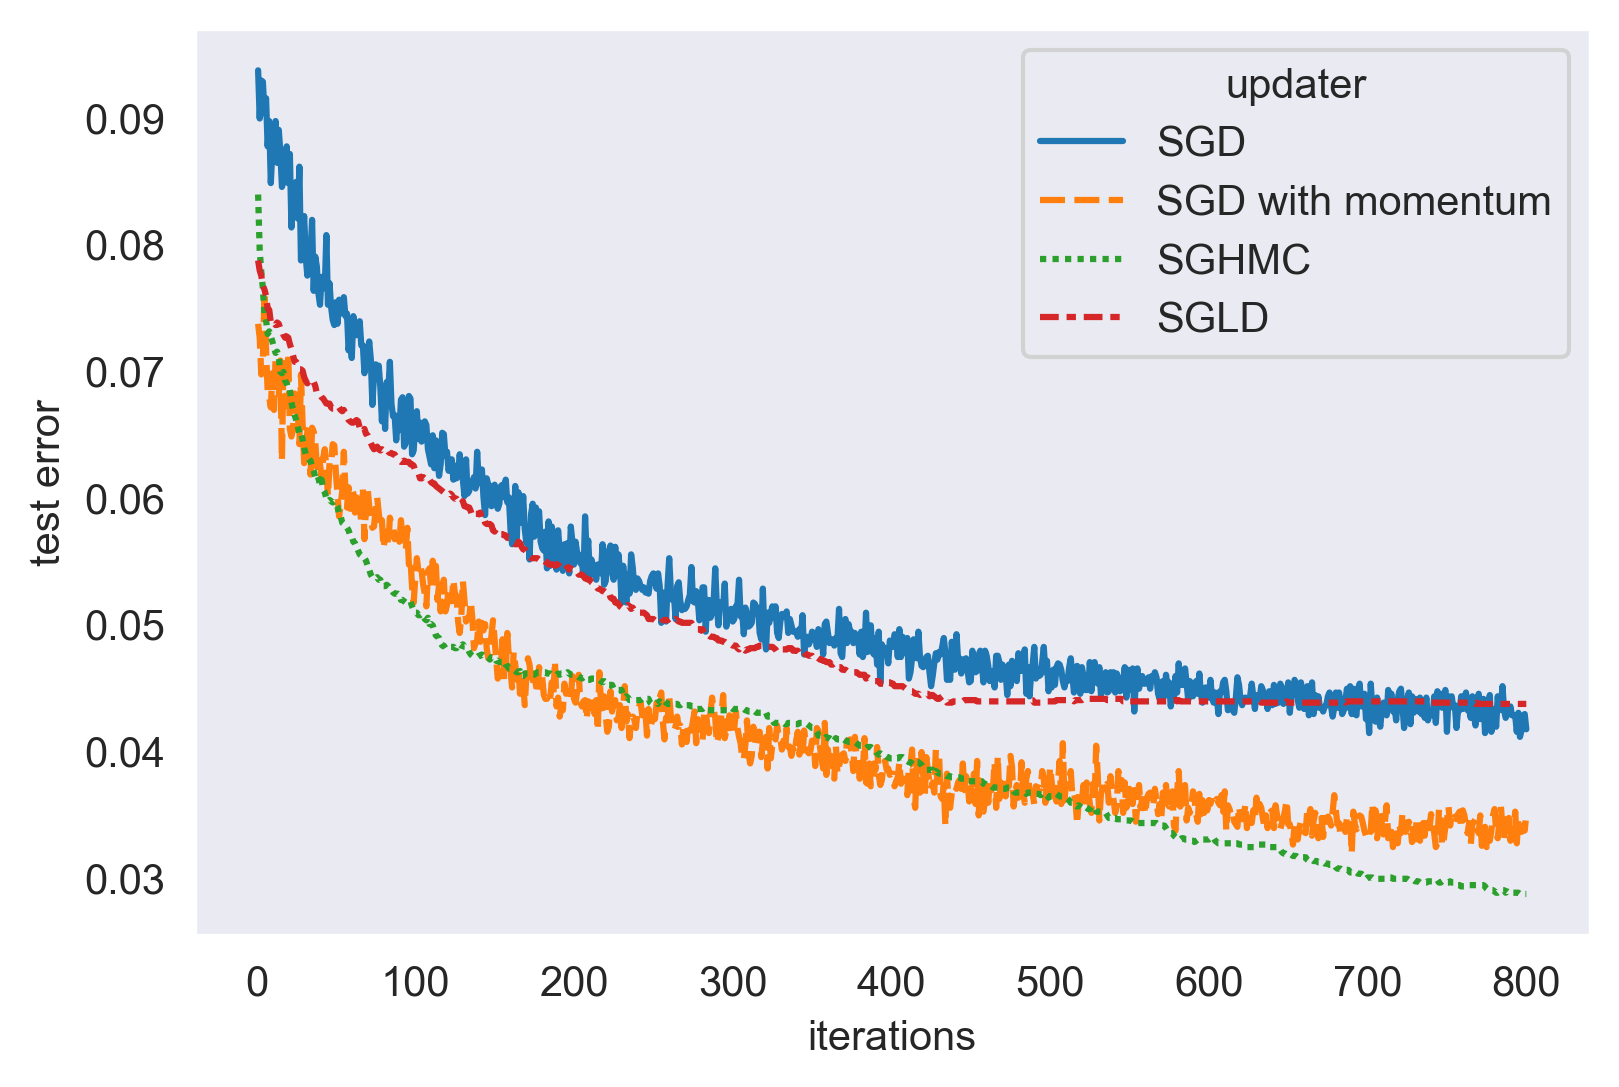
\includegraphics[width=100mm]{parts/Images/MNIST.png}
\caption{Reproducing the MNIST classification experiment from \cite{sghmc}; SGHMC ($\eta = 2.0\time10^{-6}, \alpha=0.01, \texttt{resample\_n} =0$ ), SGLD ($\eta = 4.0\time10^{-5}$), SGD ($\eta = 1.0\time10^{-5}$), SGD with momentum ($\eta = 1.0\time10^{-6}, \alpha=0.01$)}
\label{fig:MNIST}
\end{figure}
The results we get from MNIST classification align very closely with those in \cite{sghmc} and so we come to the same conclusion; the need for scalable and efficient Bayesian inference algorithms. The key benefit of BNNs is that we are not overconfident on out-of-distribution examples, Figure \ref{fig:B} illustrates that we still maintain this property when using SGHMC to approximately sample from the posterior distribution. We additionally conducted a brief comparison between Variational Inference (VI) and SGHMC in this setting, Figure \ref{fig:VI} outlines our findings.
\begin{figure}[h!]
\centering
\begin{subfigure}{.5\textwidth}
  \centering
  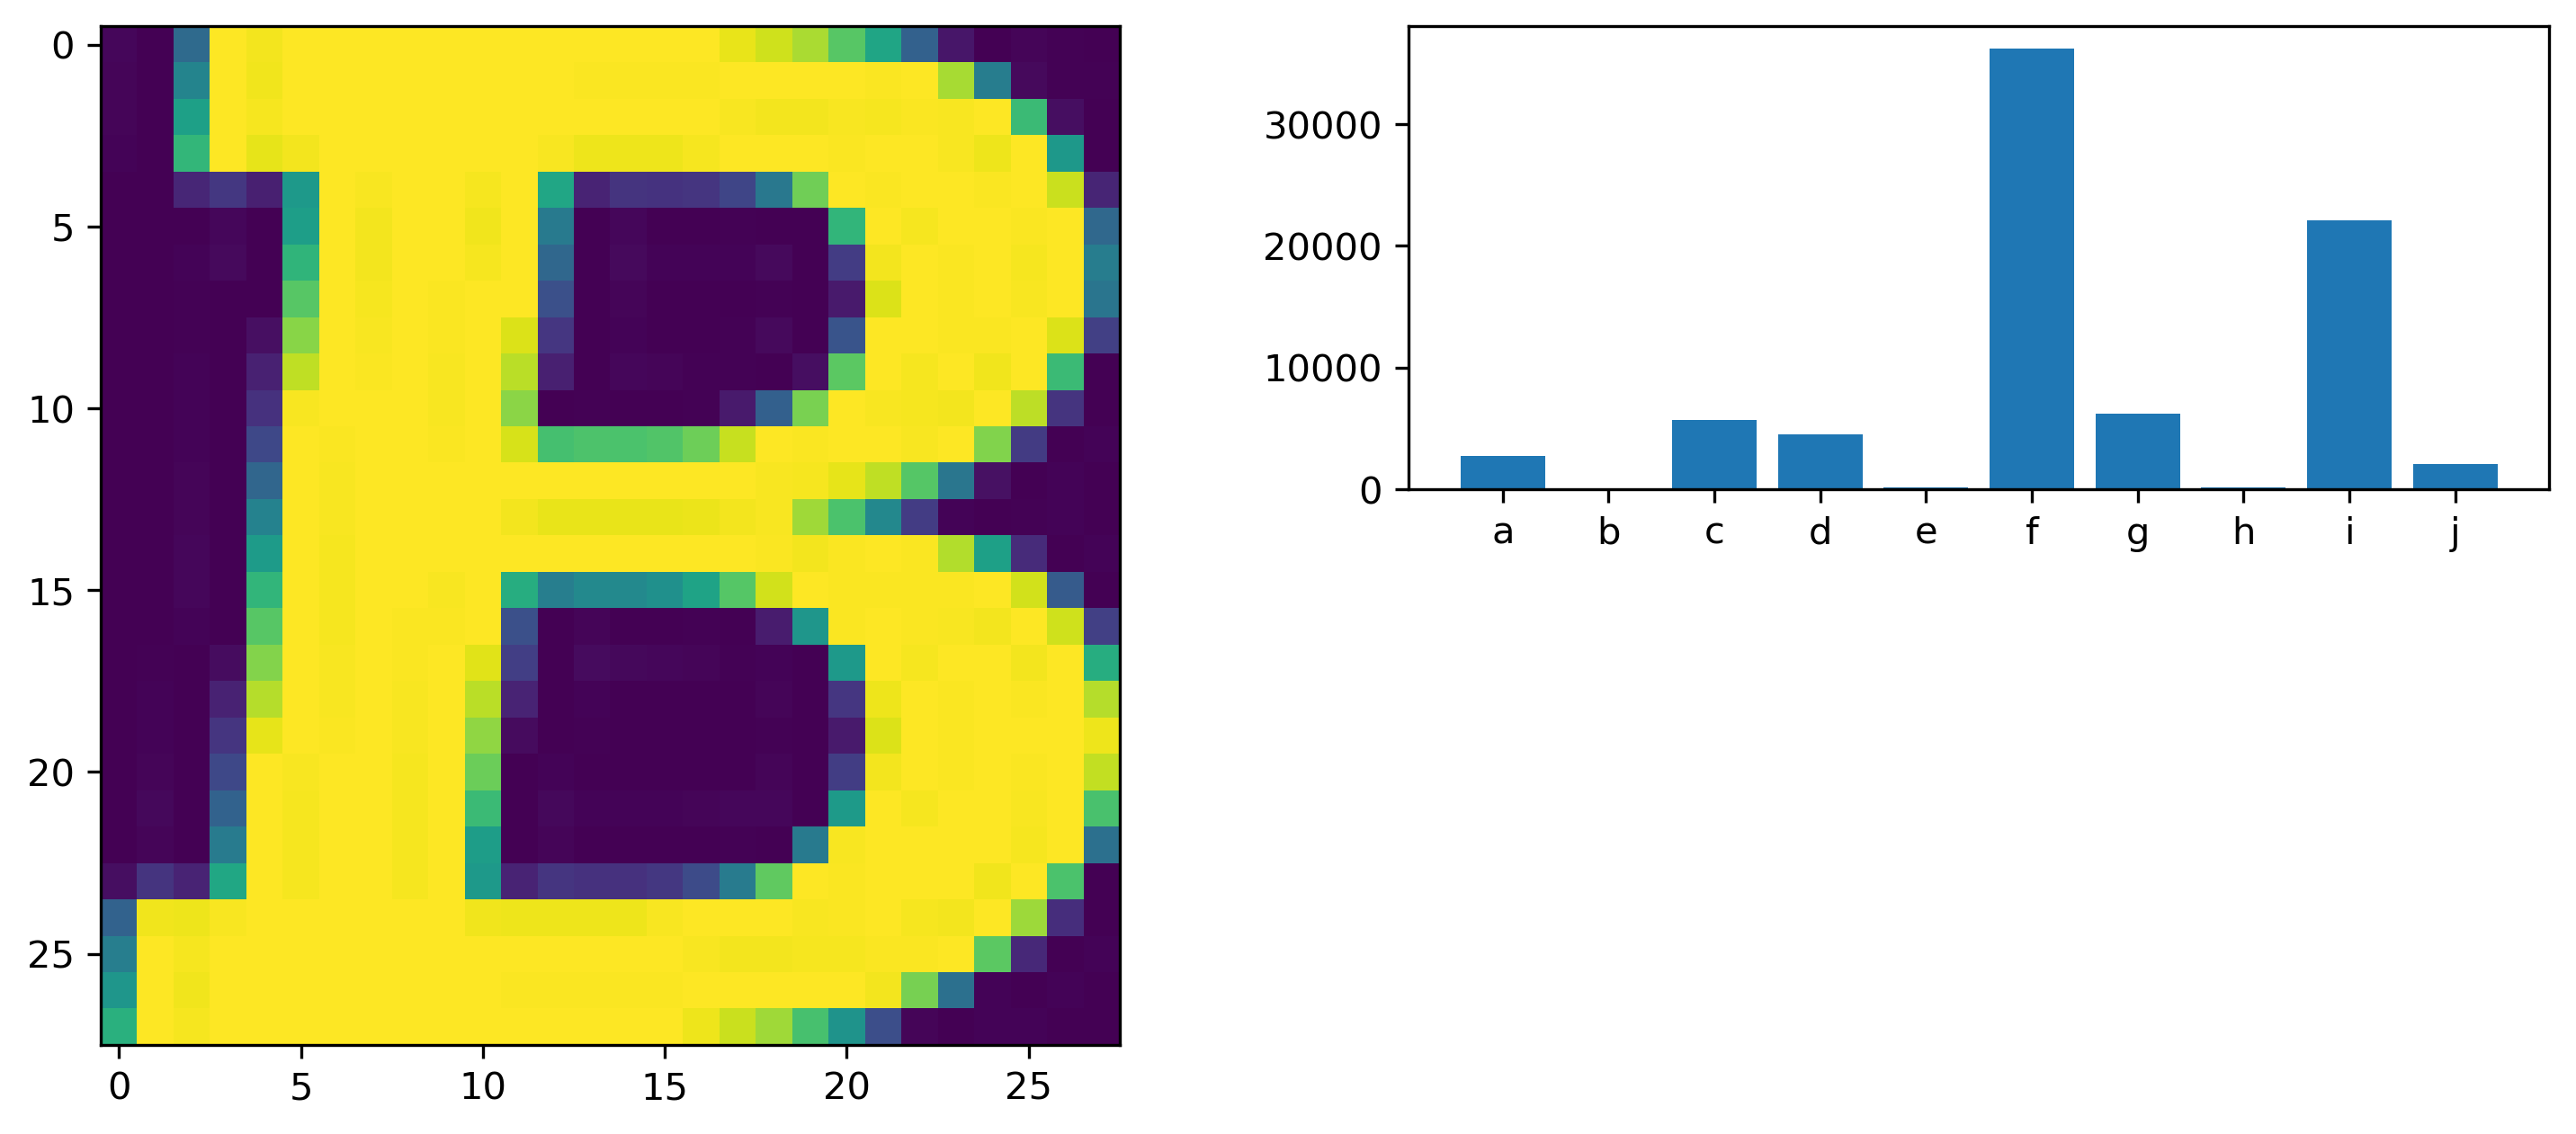
\includegraphics[width=.95\linewidth]{parts/Images/B.png}
  \caption{Uncertainty in out-of-distribution examples}
  \label{fig:B}
\end{subfigure}%
\begin{subfigure}{.5\textwidth}
  \centering
  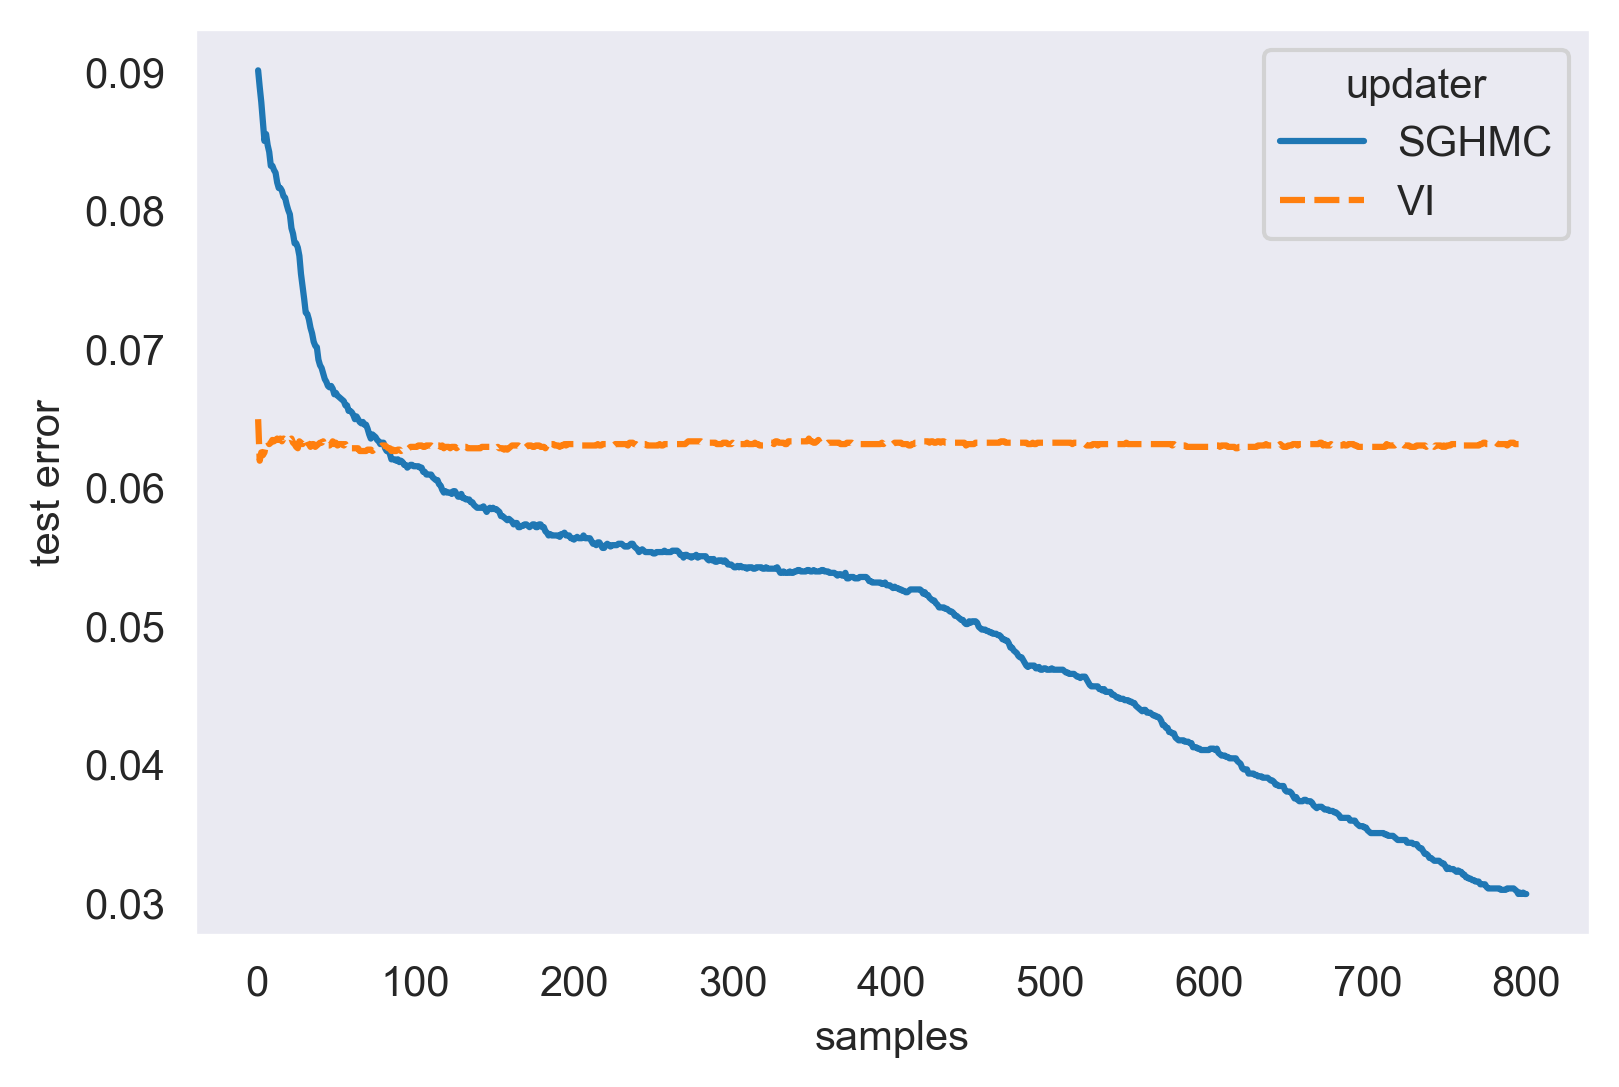
\includegraphics[width=.95\linewidth]{parts/Images/VI_SGHMC.png}
  \caption{VI and SGHMC on MNIST}
  \label{fig:VI}
\end{subfigure}
\caption{{\bf Left} (a) illustrates that we get uncertainty estimates on out-of-distribution examples. {\bf Right} (b) compares VI (Renyi ELBO, $\alpha = 0.01$, \texttt{num\_particles} $= 2$) and SGHMC ($\eta = 2.0\time10^{-6}, \alpha=0.01, \texttt{resample\_n} =0$) on MNIST. For VI we draw 80000 samples from the variational posterior $q_{\phi}$ and report the test error by Bayesian averaging. For SGHMC we do the same, except we are approximately sampling from the true posterior $p(\theta \: | D \:)$.}
\label{fig:demo}
\end{figure}
The initial results suggest that SGHMC performs better than VI in this setting, although this is not the full picture. Once VI fits the variational posterior distribution $q_{\phi}$ as closely as possible to the true posterior it takes only hundreds of samples to characterise $q_{\phi}$, whereas SGHMC requires several more samples to characterise the true posterior. In practice storing thousands of parameterisations of the same NN is very costly and so this is probably why VI is a more popular choice for Bayesian inference. 

We conclude this section by demonstrating our algorithms can be applied to other datasets and more complicated models, Figure \ref{fig:fashionMNIST} presents the results of running the same BNN architecture on FashionMNIST, and Figure \ref{fig:CIFAR10} demonstrates that our implementation of SGHMC can be used with convolutional neural networks (CNNs).
\begin{figure}[h!]
\centering
\begin{subfigure}{.5\textwidth}
  \centering
  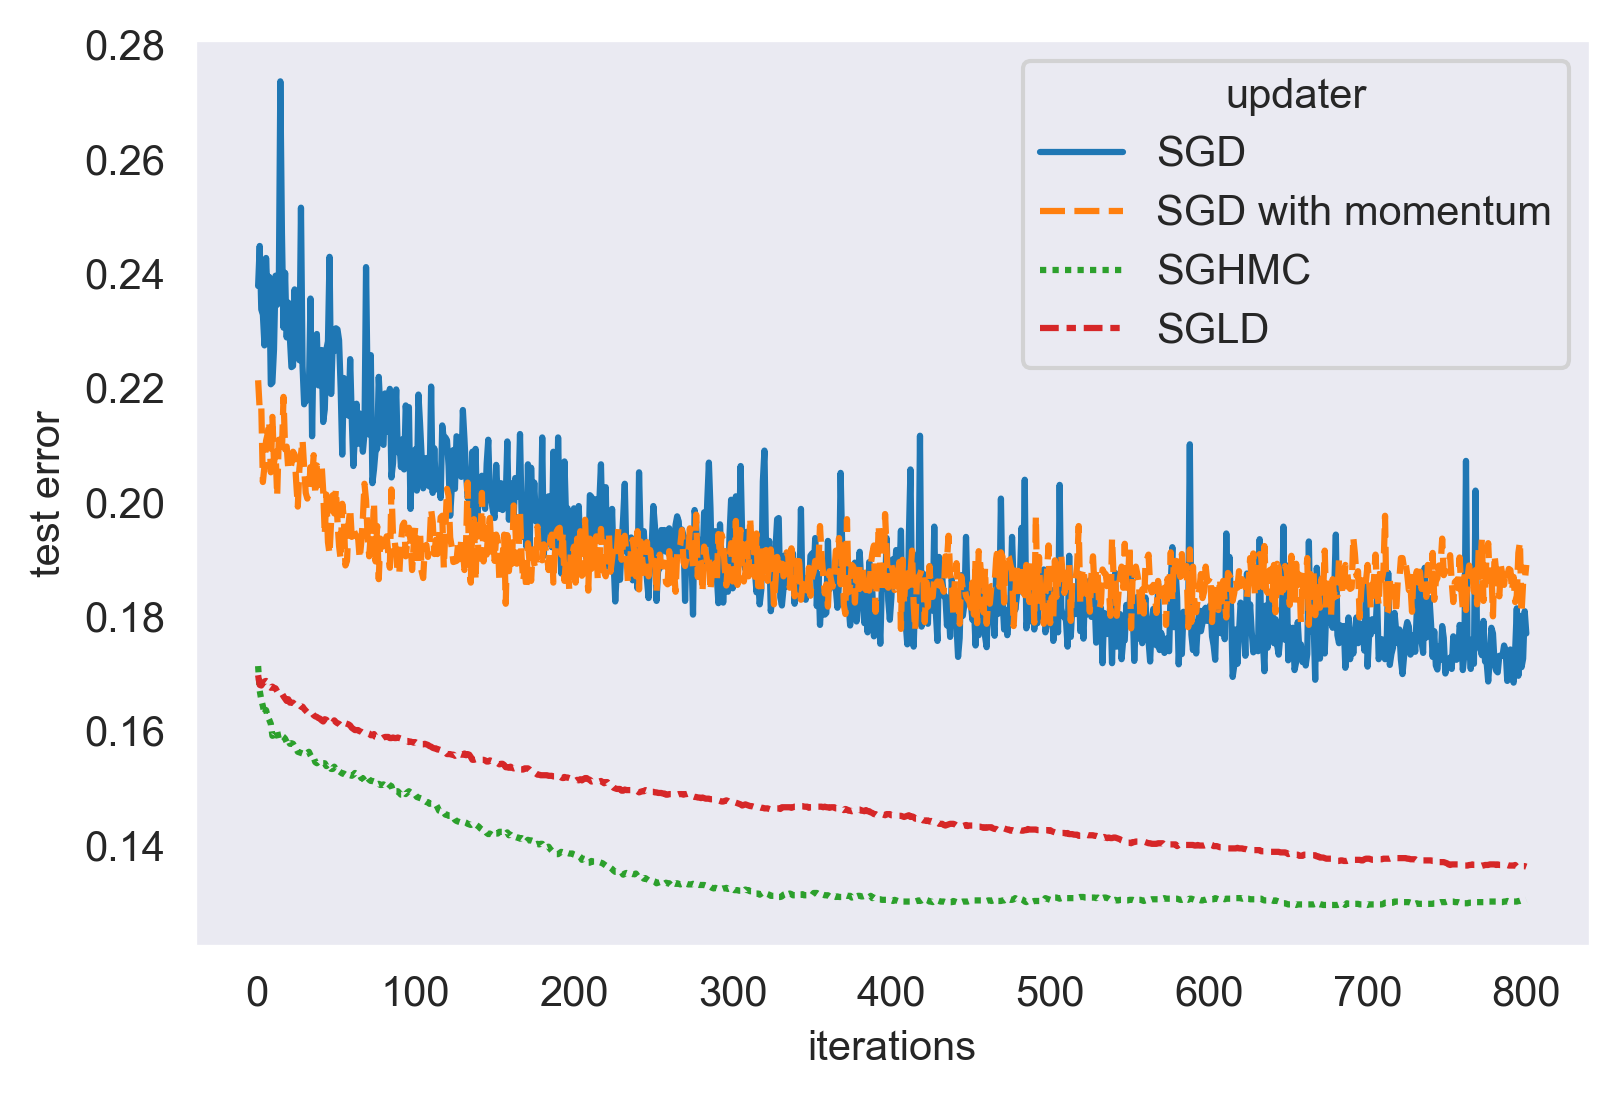
\includegraphics[width=.95\linewidth]{parts/Images/fashion-mnist.png}
  \caption{Experiment on FashionMNIST}
  \label{fig:fashionMNIST}
\end{subfigure}%
\begin{subfigure}{.5\textwidth}
  \centering
  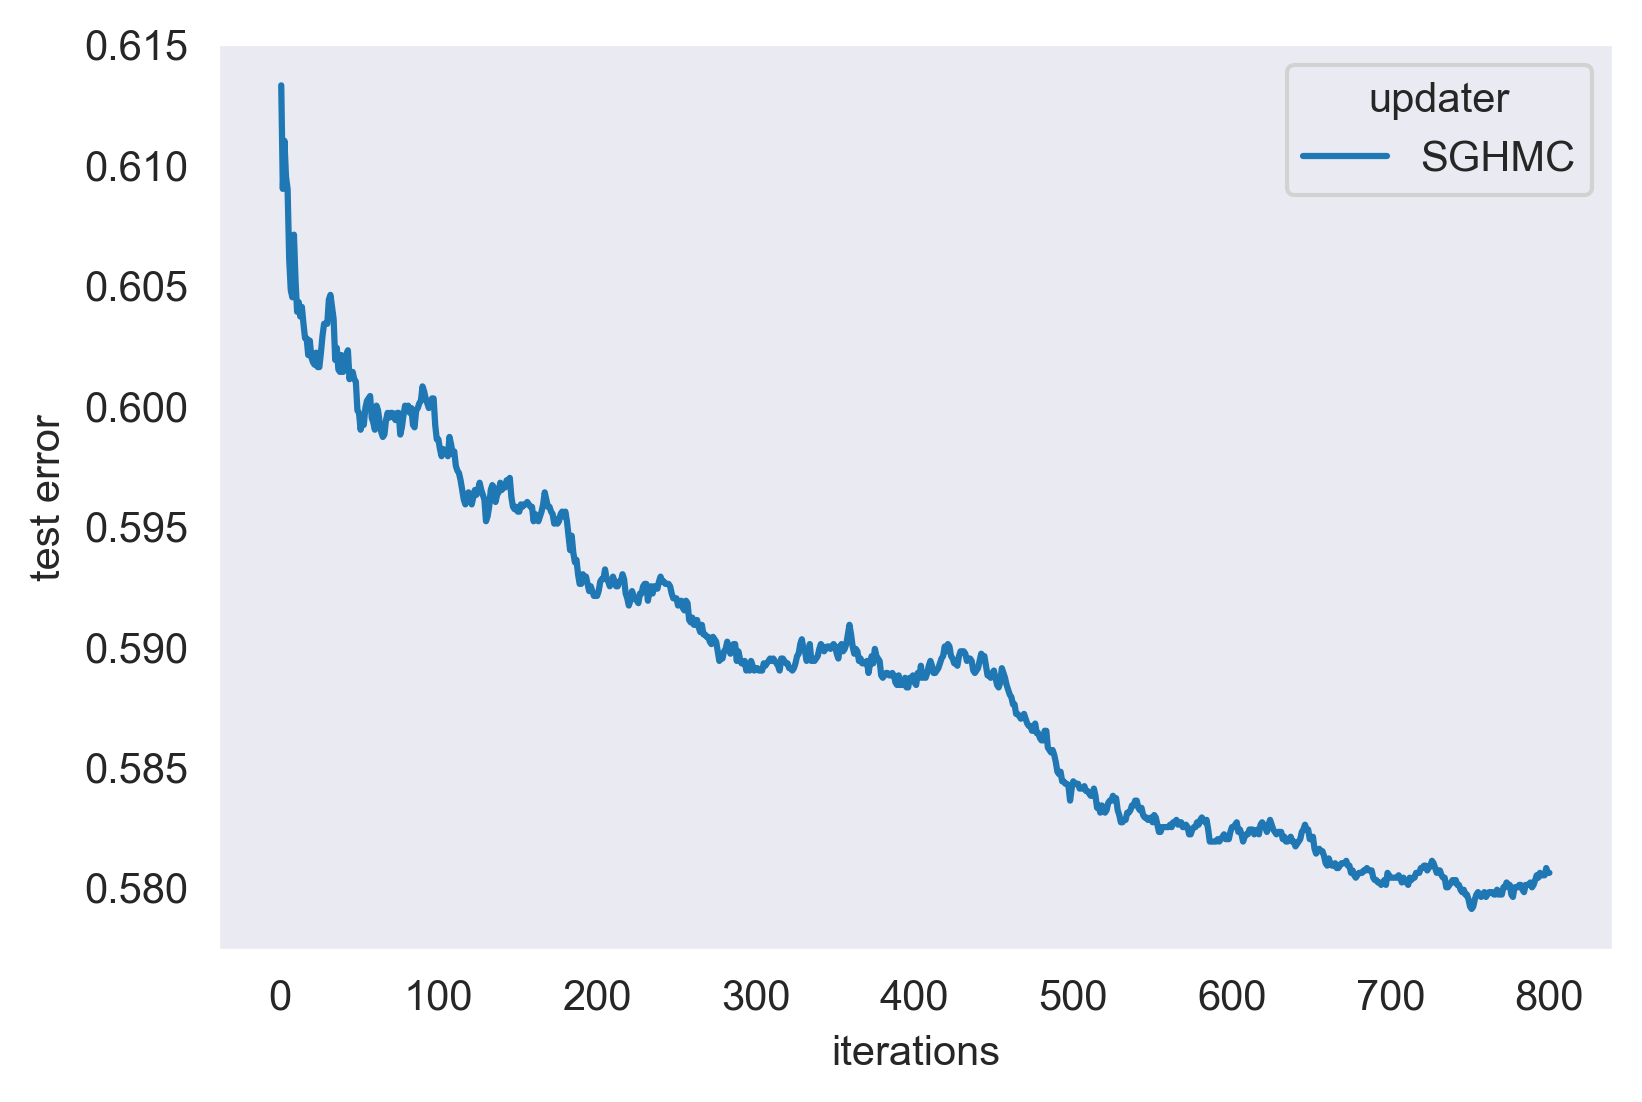
\includegraphics[width=.95\linewidth]{parts/Images/CIFAR10.png}
  \caption{Convolutional BNN on CIFAR10}
  \label{fig:CIFAR10}
\end{subfigure}
\caption{{\bf Left} (a) FashionMNIST classification; SGHMC ($\eta = 1.0\time10^{-6}, \alpha=0.01, \texttt{resample\_n} =0$ ), SGLD ($\eta = 1.0\time10^{-5}$), SGD ($\eta = 1.0\time10^{-5}$), SGD with momentum ($\eta = 1.0\time10^{-6}, \alpha=0.01$); \texttt{warmup\_epochs} $= 100$. {\bf Right} (b) Convolutional BNN with 2 convolutional layers, batch norm, max pooling and tanh activations followed by two Bayesian linear layers with tanh activation;  SGHMC ($\eta = 1.0\time10^{-6}, \alpha=0.01, \texttt{resample\_n} =0$ ) ; \texttt{warmup\_epochs} $= 150$.}
\label{fig:other-datasets}
\end{figure}